% Rafael Sartori M. dos Santos, 186154
\documentclass[brazilian,a4paper,twocolumn]{article}

% Título
\title{MC832 -- Prova 1}
\author{Rafael Sartori M. Santos, 186154}
\date{19 de novembro de 2020}

% Configuração do documento
%\setlength{\parskip}{3pt}
\usepackage[utf8]{inputenc} % tipo de documento UTF-8
%\usepackage{mathtools} % permitir expressões matemáticas
%\usepackage{breqn} % equações quebradas em várias linhas automaticamente
\usepackage{babel} % configuração da lingua portuguesa
\usepackage{caption} % para legenda de tabelas e figuras
\usepackage[
    pdfauthor={Rafael Sartori M. Santos},
    pdftitle={Prova 1 -- MC832},
    pdfproducer={LaTeX (texlive) com hyperref},
    hidelinks
]{hyperref} % para links externos (href)
\usepackage{cleveref} % para referenciar tabelas e figuras melhor
\usepackage{indentfirst} % indentação de todo primeiro parágrafo
\usepackage{graphicx} % para adicionar imagens
\graphicspath{{imgs-prova1/}} % atalho para o caminho das imagens
\usepackage{float} % para fixar posição de imagens
\usepackage{subcaption} % para imagens ficarem lado a lado
% Usamos geometry pois dá mais espaço que fullpage
%\usepackage{geometry} % alterar geometria do papel
%\geometry{a4paper,left=1.7cm,right=1.7cm,top=1cm,bottom=2.0cm} % menor margem
\usepackage{fullpage} % utilizamos uma versão com menos espaçamento nas bordas
\usepackage{verbatim} % pacote para incluir arquivos em verbatim
\usepackage{mdframed} % para enquadrar coisas
\usepackage[bitstream-charter]{mathdesign} % Mudamos a fonte para Charter BT
\usepackage[T1]{fontenc} % Mudamos a fonte para Charter BT

% Início do documento
\begin{document}

\maketitle

\section{Resumo}

O usuário acessa a internet através do celular dentro do carro que provavelmente estará se movendo, então sua conexão com a internet, que é realizada por protocolos de redes móveis, irá alternar entre diversos pontos de acesso. Essa mudança de pontos de acesso é prevista no protocolo para manter todas as conexões, evitar a perda de pacotes e age de forma natural e muitas vezes imperceptível ao usuário.

O usuário tenta acessar a página HTTP de um domínio através da aplicação de navegador, o navegador internamente faz a requisição ao servidor DNS através de uma conexão TCP ou, mais comumente nessa aplicação, utilizando o UDP para obter o endereço do servidor apontado pelo domínio. Ao recebê-lo, tenta criar uma conexão TCP com o servidor apontado pelo domínio obtido do DNS e, se obtiver sucesso, envia um pedido de página HTTP para esse endereço. O servidor então busca a página através da aplicação \textit{web} e responde ao usuário na mesma conexão criada.

O navegador, ao receber a página HTML, começa a interpretá-la e envia requisições da mesma forma ao servidor de elementos faltantes da página, que podem ser imagens, \textit{scripts}. Cada versão de HTTP trata essas requisições de forma diferente: podem utilizar conexões novas, reaproveitar a que foi utilizada para requisitar a página inicial ou ainda usar várias conexões simultâneas desde o começo, já que atualmente é comum sites HTTP pedirem mais de um arquivo por página. No caso da abertura de novas conexões, é comum o celular, o navegador ou até mesmo a rede móvel fornecer uma resposta mais rápida à uma requisição DNS que seja idêntica a uma feita anteriormente através do \textit{caching}. O servidor responde utilizando a conexão que o usuário criou ou manteve aberta e o navegador volta a interpretrar os itens recebidos, mostrando a página ao usuário dentro do carro em movimento.

Realmente é uma enorme jornada que tomamos como automática, rápida e simples, mas está bem longe de simples ou automática. Podemos ver na \cref{fig-estrutura-resumo}.

\begin{figure*}
    \centering
    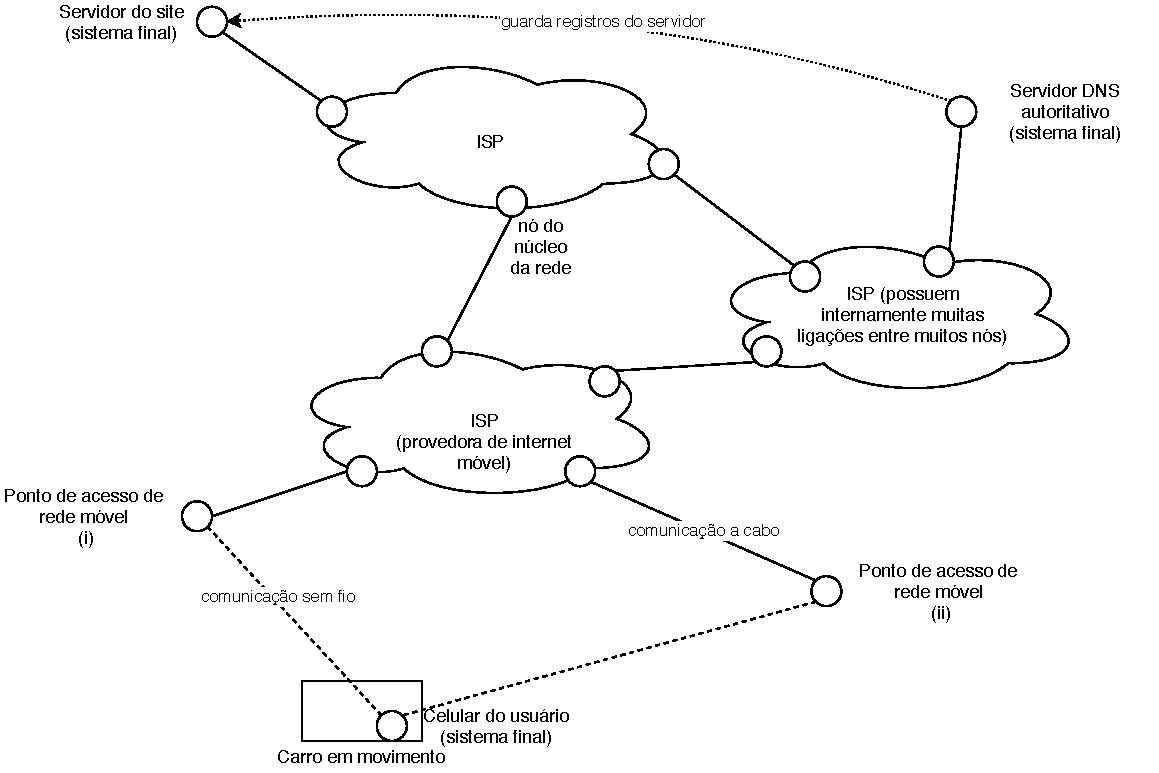
\includegraphics[width=0.9\textwidth]{prova1-figura-estrutura.pdf}
    \caption{Estrutura da rede no exemplo do resumo}
    \label{fig-estrutura-resumo}
\end{figure*}


\section{A internet e suas camadas}

A rede de computadores foi projetada com diversas camadas para encapsularmos problemas e a fucionalidade da rede, sem que o usuário precise saber de como a rede funciona ou o que ela faz para lidar com seus problemas internos. O principal modelo de rede é o modelo OSI (\textit{Open System Interconnection}) da ISO (sigla em inglês para a Organização Internacional de Normalização).

A internet é uma implementação de uma rede de computadores que foi adotada praticamente pelo mundo inteiro, interligada em vários pontos inclusive com cabos de fibra ótica que passam no fundo do oceano para ligar, por exemplo, a Europa à América. A internet difere um pouco do modelo OSI. São as camadas da internet:

\begin{itemize}
    \item{\textbf{Física:} é a camada que representa o meio físico de transporte, cada meio físico tem diferentes necessidades, limitações e capacidades;}
    \item{\textbf{Enlace:} é a camada que transmite os pacotes pelo meio físico e efetua a conferência e correção de erros de transporte (análise de sinais para diminuir interferências, impedir congestionamento do meio físico);}
    \item{\textbf{Rede:} é a camada que realiza o redirecionamento de pacotes, transportando os dados até chegar em seu destino;}
    \item{\textbf{Transporte:} é a camada que realiza multiplexação e demultiplexação dos dados para guiar o pacote ao processo certo, ela pode ou não incluir mais dados sobre o pacote para que haja conferência se todos os pacotes foram transmitidos corretamente no lado do receptor e ainda realizar a retransmissão caso haja falhas;}
    \item{\textbf{Aplicação:} a mais próxima do usuário, é a camada que envia e recebe informações de uma maneira ordenada e acordada entre o cliente-servidor através de convenções privadas ou públicas, essa camada abrange no modelo OSI as camadas \textbf{Sessão}, \textbf{Apresentação} e \textbf{Aplicação}, ou seja, a aplicação possui liberdade para executar o protocolo que quiser (seja protocolo criado exclusivamente alguma funcionalidade privada ou por protocolos muito bem estipulados por comissões internacionais para uma funcionalidade geral, pública).}
\end{itemize}

Na rede, clientes são os que iniciam a comunicação com os servidores, ou seja, um mesmo computador pode possuir aplicações clientes, aplicações servidores e aplicações que são ambos. A comunicação pode ser bilateral entre cliente e servidor, mas o início dela deve acontecer por parte do cliente, pois o servidor a priori não sabe quem deseja o quê.

Com essas camadas implementadas e interligadas formando uma rede, teremos o núcleo da rede onde os pacotes não serão interpretados senão pelas informações necessárias para determinar o destinatário e serem transmitidos de acordo. Nas bordas da rede, teremos todos os clientes e servidores, considerados sistemas finais por estarem na borda, que irão produzir e enviar pacotes, receber e interpretá-los. O núcleo da rede utiliza apenas as camadas física, de enlace e de rede, que são as necessárias para a transmissão dos dados e determinação do destino do pacote, enquanto as bordas utilizam todas, pois de fato precisam interpretar as informações transmitidas ou produzir essas informações para que a aplicação faça efetivo uso da rede.

Na internet, o endereço de um dispositivo conectado na rede é denonimado endereço IP (IP, \textit{Internet Protocol}), um número de 32 \textit{bits} para a versão 4 ou de 128 para a versão 6. Há várias regras para endereços IPs: alguns valores são reservados, alguns utilizados para redes locais e outros para redes públicas. A versão 6 também ainda não é suportada por todos os dispositivos mesmo que sua adesão tenha crescido bastante na última década.

Os usuários devem contratar provedores de serviço de internet (\textit{Internet Service Provider}, ISP) para adquirirem acesso à internet. ISPs são empresas que administram o núcleo da rede, construindo e mantendo o cabeamento necessário para isso, possibilitando conexões entre outras ISPs e todas juntas formando a rede internet que conecta o mundo todo. A ISP administrará seu endereço IP (pode ser dinâmico e mudar depois de algum tempo ou estático e quase nunca mudar), também irá providenciar os credenciais necessários para o usuário se conectar à rede de acesso, que está ligada ao núcleo da rede.

Em vários países, há leis que regulam ISPs para manter a privacidade de seus clientes, para garantir que o acesso não é privilegiado em relação a outros clientes, para garantir que a velocidade contratada é próxima à velocidade recebida pelo usuário.

A rede local, com IPs atribuídos por um roteador particular aos computadores conectados, é chamada de \textit{local area network} (LAN), a velocidade de transferência dentro da rede é apenas limitada pelo roteador, por isso é tipicamente maior que a taxa de transferência com a rede externa, chamada de \textit{wide area network} (WAN), que é a internet (onde os IPs são atribuídos pelos provedores), pois o custo de implementar uma rede de alta velocidade para todos os usuários numa rede de longa distância é maior do que numa rede local para poucos usuários e curta distância.


\subsection{Camada de aplicação}

É a camada mais dinâmica de todas porque cada aplicação no seu computador que utiliza de alguma forma a internet pode fazer uso dela como quiser (dentro das limitações impostas pela rede). Desde que o servidor consiga se comunicar com o cliente e vice-versa, qualquer protocolo vale.

Por essa aplicação ser tão dinâmica, há praticamente nenhum requisito para uma aplicação que faz uso da internet, apenas as necessidades das camadas inferiores (veremos mais tarde, os requisitos serão o endereço IP, a porta da aplicação servidor e qual protocolo de transporte deseja utilizar), a camada de transporte fará o trabalho de transmitir (e, se necessário, retransmitir) esse pacote até o destinatário correto.

Algumas aplicações essenciais para a internet que conhecemos hoje são DNS e HTTP.

\subsubsection{DNS}

O DNS ou \textit{domain name system} é um sistema que possibilita a tradução de nomes de domínios que são facilmente lembrados por humanos como \texttt{google.com} ou \texttt{unicamp.br} em endereços IP do servidor. DNS também permite vários tipos de entradas: \texttt{A}, \texttt{AAAA}, \texttt{MX}, \texttt{ALIAS}, \texttt{CNAME} etc. cada uma com sua funcionalidade específica que permite diferentes tipos de requisições de serviço (servidor de e-mail ser diferente do seu servidor \textit{web} mesmo que o domínio seja o mesmo, ou ainda fazer balanço de requisições através de uma mudança de entrada \texttt{A} para um servidor secundário quando o servidor primário começar a ficar sobrecarregado, por exemplo).

A estrutura do DNS para resolução de nomes é hierárquica: há, no topo, os servidores raiz que respondem os servidores \textit{top level domain} (TLD, que são os domínios específicos de países, \texttt{.br}, \texttt{.ar}, ou os genéricos como \texttt{.org}, \texttt{.com}, \texttt{.gov}). Os servidores TLD respondem os servidores autoritativos, que são os que guardam de fato as entradas para o domínio buscado. Todo servidor autoritativo possui um servidor espelho que servirá de \textit{backup}, um servidor secundário.

Como a estrutura é hierárquica, poderia haver enorme sobrecarga das instâncias dos servidores raiz, então há diversos servidores que realizam o \textit{caching} das pesquisas já feitas e distribuem os pedidos entre os usuários. Muitas ISPs possuem seu próprio servidor DNS desse tipo, chamados de DNS local. Além da distribuição, há diferentes tipos de consultas DNS: recursiva (responde fazendo a busca pelo servidor raiz quando não possui \textit{cache} da requisição), iterativa (responde com o servidor DNS autoritativo sobre o domínio, para obter a resposta atualizada apropriada) e não recursiva (busca registros onde o servidor é autoritativo ou possui \textit{cache}, mas não consegue responder caso contrário).

Seu computador, roteador também podem possuir servidores DNS locais para melhorar ainda mais a latência de respostas em \textit{cache}.

As diversas aplicações cliente e servidor do DNS implementam um protocolo de comunicação comum, assim mesmo implementações de cliente ou servidor distintas conseguem se comunicar por uma estrutura comum de pacotes.

\subsubsection{HTTP}

Como DNS, HTTP também possui enorme quantidade de implementações de um protocolo de comunicação que é comum. Essencialmente, HTTP serve para que clientes consigam pedir arquivos \textit{hypertext} (texto estruturado que possui ligações para outros arquivos) e arquivos de mídia necessários para apresentação dessa estrutura. Esses arquivos que formam páginas exibidas ao cliente podem conter referências a outras páginas. Páginas de um mesmo domínio são chamados de site e a ligação entre páginas de diferentes sites formam a \textit{world wide web} através de uma cadeia enorme de páginas interligadas.

HTTP historicamente foi associado através dos navegadores ao HTML, um formato de texto hierárquico que descreve visualmente uma página. Hoje esse formato ganhou muitas funcionalidades dinâmicas (que não requerem recarregar a página a cada clique) através de \textit{scripts} e ficaram mais bonitas com arquivos que descrevem estilos (\textit{Cascading Style Sheets} ou CSS).

O protocolo sofreu algumas reformas logo após sua criação mas passou muito tempo na mesma versão (\texttt{HTTP/1.1}) até a adoção ainda crescente da segunda versão, o \texttt{HTTP/2.0}. Com a nova versão, agora há algumas formas de tratar conexões:

\begin{itemize}
    \item \textbf{HTTP não persistente:} nesse modo, após o envio de um único objeto, a conexão é fechada e, caso exista a necessidade de pedir outro objeto, uma nova conexão deve ser criada;
    \item \textbf{HTTP persistente:} a conexão é mantida para evitar o \textit{overhead} de criar uma nova quando há a necessidade de pedir outro objeto, diminuindo o tempo para página carregar;
    \item \textbf{HTTP com paralelismo:} várias conexões são criadas para pedir em paralelo diversos objetos (é comum HTML possuir a necessidade de vários objetos serem carregados) e ainda é possível fazer isso com persistência;
    \item \textbf{HTTP com multiplexação:} a nova versão do HTTP (\texttt{HTTP/2.0}) permite que uma única conexão seja utilizada, o diferencial é que a requisição será quebrada em partes, \texttt{HEADERS} e \texttt{DATA}, enquanto permite o envio e recebimento simultâneo entre cliente e servidor através de \textit{streams}. É uma abordagem que diminui o tempo de carregamento inclusive em condições de baixa estabilidade de rede pois não há a necessidade de várias conexões para se pedir vários arquivos simulteamente. Também é muito útil nos sites modernos que fazem uso de \textit{scripts} para se comunicar com o servidor (como Facebook, Instagram, sites cujas páginas são dinâmicas ao invés de carregar a página totalmente no primeiro acesso e após cada clique).
\end{itemize}


\subsection{Camada de transporte}

Computadores podem possuir diversas aplicações, cada uma pode se comunicar com diversos servidores tanto simultaneamente quanto linearmente. Por isso, essa camada é geralmente implementada pelo sistema operacional, que deve organizar todos os pacotes para que nada seja perdido ou passado à aplicação errada por engano.

Nessa camada, os aplicativos podem escolher entre os protocolos de transporte:

\begin{itemize}
    \item \textbf{TCP (\textit{Transmission Control Protocol}):} esse protocolo utiliza uma conexão mantida entre cliente e servidor e garante o recebimento integral e correto da sequência de mensagens através do encapsulamento do pacote com informações sobre cada pacote, como número sequencial, controle de fluxo, confirmações de recebimento;
    \item \textbf{UDP (\textit{User Data Protocol}):} não utiliza conexão, os pacotes são enviados de forma direta, sem qualquer espécie de ``preâmbulo'' e não é previsto verificação de recebimento e de fluxo, ou seja, pacotes perdidos não serão necessariamente reenviados.
\end{itemize}

É importante ressaltar que, apesar do UDP não suportar esses recursos que TCP proprõe, é possível implementar essas funcionalidades de TCP em UDP através da camada de aplicação. Também que não é previsto controle de sessão em nenhum dos protocolos, pois isso é de controle da aplicação.

Para o computador permitir várias aplicações diferentes se comunicarem em rede, é necessário atribuir valores únicos a cada comunicação da aplicação, de uma forma que seja possível o sistema operacional direcionar pacotes corretamente às aplicações. Com essa necessidade, o recurso que possibilita realizar essa função é chamado de porta, um número que identifica qual processo irá receber esse pacote. Na aplicação servidor, temos uma porta fixa, de forma que qualquer cliente do mundo que saiba o endereço IP e a porta conseguirão enviar pacotes à aplicação. Já na cliente, a porta geralmente é um número aleatório em que o sistema guarda numa tabela ou ainda, para facilitar o trabalho do sistema, é o próprio número do processo da aplicação.

\subsubsection{Início da comunicação}

Para iniciar a camada de transporte, o sistema operacional precisa receber da aplicação o endereço do servidor, a porta que espera pacotes na aplicação servidor e o protocolo de transporte utilizado. O sistema operacional então cria um \textit{socket} para receber e enviar as informações recebidas pela rede. \textit{Sockets} são estruturas para a comunicação entre a aplicação e o sistema operacional ou até entre diferentes aplicações, permite a leitura e escrita a depender das permissões definidas e geralmente são mantidas através de \textit{buffers}.

Para envio dos dados, a camada de transporte precisa fazer a multiplexação (cada aplicação imagina que possui a rede toda para si, mas na verdade a rede é compartilhada). A multiplexação é receber os pacotes das aplicações através dos diversos \textit{sockets}, adicionar os dados necessários para cada protocolo de transporte e colocá-los no \textit{buffer} de rede para serem enviados pela camada de rede.

Já para o recebimento, a camada de transporte efetua a demultiplexação (os passos opostos à multiplexação) que é receber o pacote através do \textit{buffer} de rede, verificar o recebimento integral e correto do pacote através das informações adicionadas pelos protocolos de transporte e depois colocá-lo no \textit{socket} representado pela porta de destino.

Cada protocolo verifica o pacote e adiciona ou analisa informações específicas do protocolo para que ele seja executado de forma correta.


\subsubsection{Comunicação utilizando UDP}

O UDP é o mais simples, adiciona a porta da aplicação remetente e a da destinatário no pacote, também inclui o tamanho do pacote e uma soma de verificação. A soma de verificação possibilita identificar pacotes transferidos incorretamente e filtrá-los de serem enviados à aplicação e também está presente em TCP.

Essas informações são suficientes, não há mais nenhum outro controle, esses recursos devem ser providos pela aplicação se necessário. Com isso, temos um protocolo em que, se o pacote foi recebido corretamente, ele é enviado à aplicação correspondente. Caso contrário, se o pacote foi recebido incorretamente, será descartado; se não foi, não será reenviado a não ser que a aplicação implemente recursos para isso acontecer.


\subsubsection{Comunicação utilizando TCP}

Já em TCP, os recursos precisam de maior quantidade de informações para serem executados, como diversas \textit{flags} para controle de fluxo, um número sequencial para cada pacote e ainda um valor do último pacote recebido, que permite identificar pacotes perdidos. Para suportar essas funcionalidades que juntas provém confiabilidade à comunicação, é necessário um sistema na camada de transporte bem mais robusto do que o UDP.

TCP, por usar uma conexão, precisa de alguns passos para iniciá-la através de um acordo de 3 vias (\textit{three-way handshake}). Antes de tudo, o servidor deve estar preparado com um \textit{socket} aberto no sistema operacional para receber pacotes em alguma porta específica. Como apenas o cliente tem como requisitar a conexão, já que o servidor não saberia quem deseja se conectar, ele envia o primeiro pacote, que possui a \textit{flag} \texttt{SYN} (\textit{synchronize}). O servidor responde o \texttt{SYN} com um \texttt{SYN+ACK} (\textit{synchronize acknowledgement}) reconhecendo o pedido do cliente. O cliente confirma o recebimento do servidor ter aceito através de um \texttt{ACK} e a conexão pode iniciar entre os dois através da camada de aplicação. Qualquer falha ou falta de resposta num tempo esperado irá resultar na conexão fechada para ambos.

O número sequencial dos pacotes inicia logo durante o \textit{handshake}, cada pacote usada a partir disso (inclusive na conexão) incrementará relativo ao cliente e ao servidor. O cliente mandará \texttt{ACK} com o número sequencial do último pacote recebido do servidor e vice-versa. Com isso, conseguimos detectar quando um pacote não chegou corretamente: um dos lados enviaria pacotes, mas o último recebido pelo outro lado se mantém num número de sequência anterior ao do que falhou (recebemos vários \texttt{ACK} com valor anterior ao que estamos enviando atualmente ou não receberemos nenhum e o tempo de espera terá excedido -- \textit{timeout}), assim é possível reenviar todos os pacotes incluindo os que não foram ainda reconhecidos. Ou seja, utilizando TCP, os pacotes só saem do \textit{buffer} da camada de transporte quando são reconhecidos.

Para mantermos esses pacotes dessa forma, é necessário um lado tomar ciência do tamanho do \textit{buffer} do outro através do \textit{window size} (tamanho da janela), evitando congestionamentos e perdas de pacotes que poderiam ser evitadas controlando o fluxo. Todo pacote enviado conterá o tamanho atual disponível que o destinatário possui para receber (\texttt{rwnd}, \textit{receiver window}) e o tamanho disponível para enviar antes de receber um \texttt{ACK} (\texttt{cwnd} \textit{congestion window}). Ao reconhecer um pacote através do \texttt{ACK}, se era o pacote esperado, libera-se alguns \textit{bytes} no \textit{buffer} e a janela se move, permitindo recebimento de mais dados no local desse pacote que foi confirmado.

A \textit{flag} \texttt{ACK} suporta pular os números de sequência já reconhecidos corretamente até o último recebido, ou seja, é acumulativo. Se um usuário envia de uma vez 4 pacotes de números sequenciais, por exemplo, o servidor pode responder com \texttt{ACK} apenas do último e o cliente liberará os 4 pacotes da janela. Porém isso também serve para quando o pacote de reconhecimento do servidor falhou, pois o usuário enviará novamente no mínimo 1 até todos os 4 pacotes depois desse falso \textit{timeout} e o servidor responderá com um segundo \texttt{ACK} de todos, talvez até dispensando o envio dos pacotes que não foram ainda reenviados por engano.

Para indicar que um pacote chegou fora de ordem, o recebidor envia \texttt{ACK}s duplicados com o número de sequência do último pacote que chegou em ordem, fazendo com que o outro lado perceba mais rapidamente um pacote faltante ao invés de um atraso incomum.

Junto com o tamanho de janela, TCP utiliza alguns recursos de regulação de congestionamento para permitir o maior \textit{throughput} possível, esses recursos respeitam \textit{additive increase, multiplicative decrease}, tornando a rede mais responsiva. Para adiquirir velocidade inicialmente, TCP utiliza \textit{slow start}, o número de pacotes enviados e/ou o tamanho deles inicialmente é o mínimo para conexões dentro daquela rede, mas cresce a cada \textit{round-trip time} (RTT, tempo de ida e volta, que é indicado pelo recebimento do \texttt{ACK}, ou seja, a soma do tempo do pacote caminhando a rede, sendo reconhecido e de volta do pacote de reconhecimento), dobrando a quantidade de informação enviada (\texttt{cwnd}) quando receber todos os reconhecimentos. Quando atingir \texttt{ssthresh} (\textit{slow start threshold}), outro método de evitar congestionamento é utilizado.

No outro modo, aumentamos a quantidade de dados linearmente até que o outro lado deixe de receber algum pacote (indicado por um \texttt{ACK} duplicado ou por um tempo longo sem receber reconhecimento de recebimentos), daí atualizaremos \texttt{ssthresh} para a metade do valor utilizado antes de chegar no congestionamento e podemos ou recomeçar o \textit{slow start} ou tentar manter a taxa de envio iniciando do \texttt{ssthresh} para reenviarmos pacotes que não foram reconhecidos e continuarmos com novos.

Para manter a internet atual, é importante que novos protocolos de transmissão não demandem mais da rede do que o TCP, pois poderia causar um colapso de congestionamento (quando a rede está tão congestionada que efetivamente limita qualquer comunicação útil), essa responsabilidade é chamada de \textit{TCP fairness}.


\subsection{Camada de rede}

Essa camada ficará responsável por distribuir os pacotes aos respectivos destinatários corretamente, fazendo o roteamento e encaminhamento. É aqui que é utilizado o protocolo da internet (IP) nas suas versões 4 e, ainda em adoção, 6.

O \textit{internet protocol} possui um \textit{header} próprio para permitir que os pacotes sejam enviados ao destinatário corretamente. Todos os pacotes vindos da camada de transporte podem ser encapsulados para serem distribuídos pelo IP. As informações necessárias no cabeçalho para um pacote IPv4, por exemplo, são:

\begin{itemize}
    \item a versão do protocolo utilizada;
    \item o tamanho do \textit{header}, necessário pois pode possuir tamanho variável (seção de opções que é opcional);
    \item um campo para determinar o tipo de serviço, melhorando a transmissão do pacote para prover melhor qualidade de serviço possível;
    \item notificação de congestionamento de rede;
    \item tamanho total do pacote (ele pode ser fragmentado pela rede ou pelo remetente, há valores mínimos para a fragmentação);
    \item identificação (facilitar transporte de pacotes fragmentados ou de uma mesma fonte);
    \item algumas \textit{flags} e informações sobre fragmentação;
    \item \textit{time to live} (número máximo de nós que deve passar antes de ser cancelado, evitando ficar em circulos);
    \item protocolo utilizado nos dados do pacote;
    \item soma de verificação do próprio \textit{header};
    \item endereço IP do remetente e destinatário;
    \item campo opcional para opções.
\end{itemize}

Ao deixar o remetente, o pacote recebe (geralmente através do sistema operacional, que também geralmente controla a camada de transporte) o cabeçalho IP para ser transmitido pela rede, onde será roteado ou encaminhado de nó em nó pelo núcleo da rede seguindo algum algoritmo de roteamento até chegar no destinatário, onde o cabeçalho é removido e os dados são passados para a camada de transporte.

Os pacotes que não passam pela soma de verificação são descartados. No centro da rede, várias provedoras de internet (ISPs) precisam interagir de maneira ordenada para conseguir garantir que os pacotes consigam chegar aos seus destinatários.

Entre cada nó da rede, incluindo remetente e destinatário, os dados precisarão ser colocados na camada de enlace para a transmissão ocorrer de fato.


\subsection{Camada de enlace e física}

Na camada de enlace, cada pacote no \textit{buffer} deverá respeitar a camada física, que possuem limitações específicas a depender da tecnologia de cada trecho entre os nós. Mais informações sobre o pacote podem ser adicionadas dependendo de cada meio físico, para evitar erros de transmissão ou ainda informações suficientes para saber corrigi-los. Junto com a camada física, é uma camada bastante especializada que possui muitos protocolos para cada tipo de transmissão, pois variam quanto a taxa de transmissão, taxa de erros, possibilidade de envio e recebimento simultaneos etc.

Nessas camadas, por serem onde ocorre de fato a comutação de pacotes, ou seja, a transmissão dos pacotes entre os nós da rede, são as que mais gastam tempo. O atraso nodal é o tempo total em que o pacote fica no nó (assim que entra até ter acabado de chegar no próximo nó). Temos alguns tipos de atraso:

\begin{itemize}
    \item \textbf{Atraso de processamento:} tempo para o nó ler o cabeçalho do pacote e determinar onde deve ser enviado, esse valor é pouco influenciado pela camada física utilizada. Quando um nó utiliza um controle externo para roteamento, esse tempo pode ser maior do que um roteamento individual ou descentralizado;
    \item \textbf{Atraso de fila:} a taxa de transmissão pode ser menor do que a quantidade de dados recebidos na fila, fazendo com que esse tempo seja muito grande e até fazendo pacotes serem descartados pela idade ou, eventualmente, pelo \textit{buffer} estar cheio. É o tempo em que o pacote aguarda sua vez para ser transmitido;
    \item \textbf{Atraso de transmissão:} tempo utilizado para colocar os dados de fato no meio físico, pode ser alto quando o meio possui baixa capacidade de transmissão ou ainda alto \textit{overhead} para a transferência (sem fio, por exemplo, em que podemos colocar várias informações redundantes pra auxiliar a remontagem do sinal devido perdas e interferências);
    \item \textbf{Atraso de propagação:} podemos ter um tempo grande por ser transmitido por grandes distâncias (internacionalmente, por exemplo).
\end{itemize}

Cada tipo de construção física possui diferentes capacidades de transmissão (ou vazão de dados) e diferentes probabilidades de ocorrer perdas devido transmissão (perdas que acontecem quando o pacote é corrompido na transmissão de forma irrecuperável).

\end{document}
